\chapter{Parte II}

\section{Análise do problema}

Na segunda parte é proposto ao grupo simular a gestão da empresa W\&W por um
período de 200 dias, recorrendo ao software "Jogo da Distribuição", facultado
com o enunciado do trabalho. O objetivo será maximizar o lucro total durante
o período especificado, utilizando a política de encomenda determinada na parte
anterior.

\section{Resultados obtidos}

\subsection{Nível de \emph{stock}}

As seguintes tabelas apresentam a evolução do nível de \emph{stock} a cada 40 dias de operação: 

\begin{table}[htpb]
\begin{center}
\begin{tabular}{cc}
\toprule
Dia & Stock	 	\\ \midrule
40 & 146                \\ 
80 & 116                \\ 
120 & 103               \\ 
160 & 107               \\ 
200 & 77     		\\ 
\bottomrule
\end{tabular}
\end{center}
\caption{Nível de stock no armazém}
\label{tab:tabela1}
\end{table}



\begin{table}[htpb]
\begin{center}
\begin{tabular}{cc}
\toprule
Dia & Stock	 	\\ \midrule
40 & 12                 \\ 
80 & 17                 \\ 
120 & 8                 \\ 
160 & 10                \\ 
200 & 25     		\\ 
\bottomrule
\end{tabular}
\end{center}
\caption{Nível de stock na loja 1}
\label{tab:tabela2}
\end{table}



\begin{table}[htpb]
\begin{center}
\begin{tabular}{cc}
\toprule
Dia & Stock	       \\ \midrule
40 & 6                 \\ 
80 & 1                 \\ 
120 & 13               \\ 
160 & 30               \\ 
200 & 16     	       \\ 
\bottomrule
\end{tabular}
\end{center}
\caption{Nível de stock na loja 2}
\label{tab:tabela3}
\end{table}



\begin{table}[htpb]
\begin{center}
\begin{tabular}{cc}
\toprule
Dia & Stock	 	\\ \midrule
40 & 17                 \\ 
80 & 16                 \\ 
120 & 6                 \\ 
160 & 14                \\ 
200 & 9     		\\ 
\bottomrule
\end{tabular}
\end{center}
\caption{Nível de stock na loja 3}
\label{tab:tabela4}
\end{table}




\subsection{Saldo Acumulado}

No gráfico abaixo está representada a evolução do saldo acumulado durante os 200
dias de jogo:

\begin{figure}[<+htpb+>]
	\centering
	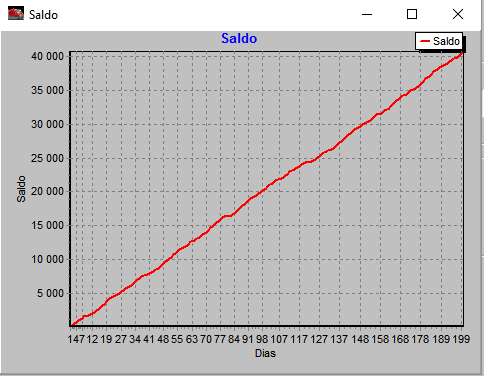
\includegraphics[scale=0.75]{./report-TP2/img/saldo.png}
	\caption{Saldo acumulado no final do jogo}
\label{fig:figure1}
\end{figure}


\newpage

\subsection{Estratégia de jogo}

No dia inicial o \emph{stock} do armazém foi inicializado em 125 unidades,
e o \emph{stock} de cada uma das lojas a 25 unidades. A política de encomendas
seguida tanto para as lojas como para o armazém corresponde à política
determinada na parte I para cada entidade:

\begin{itemize}
	\item Política de encomendas para o armazém
		\begin{itemize}
			\item $q = 276$ unidades;
			\item $S = 118$ unidades;
			\item Frequência de encomenda: 37 dias;
		\end{itemize}
	\item Política de encomendas para as lojas
		\begin{itemize}
			\item $q = 17$ unidades;
			\item $S = 5 $ unidades;
			\item Frequência de encomenda: 7 dias;
		\end{itemize}
\end{itemize}

A política de Nível de encomenda foi seguida à risca durante o jogo. Tanto para
o armazém como para as lojas, sempre que o nível de inventário descia abaixo de
\emph{S}, ou o número de dias desde o último pedido igualava o valor de frequência de
encomenda, era simulada a encomenda de \emph{q} unidades de artigo para a entidade
correspondente. Terminados os 200 dias, foi obtido um saldo final de
aproximadamente 40705 euros. O uso dos resultados obtidos na Parte I permitiram
atingir facilmente um saldo final considerável, o que comprova a utilidade dos
processos matemáticos utilizados para modelar a gestão do nível de inventário.




